% Appendix D

% variables
\newcommand{\appdird}{appendices/plots/appendixD}

\chapter{Particle tracking} % Main appendix title

\label{AppendixD} % For referencing this appendix elsewhere, use \ref{AppendixC}

%\section{Micromegas}
%\label{appD:sec:mm}


\section{Momentum reconstruction}
\label{appD:sec:mom-reco}

Momentum reconstruction is performed in two different ways in NA64. The first one consist in a simple solution based on the expected curvature of the charged particles when it enters the magnetic field. As the momentum of the primary particle is generally very high compared to its mass, this can be safely ignored. The particle can be assumed to travel in a line outside the magnets, whereas inside it the trajectory corresponds to a circle tangent to the particle entrance line. The radius of the circle is easy in the relativistic limit:

\begin{equation}
  \label{eq:gyro-radius}
  r_c = 3.3 \times \frac{p}{\left|q\right|B}
\end{equation}

where $\left|q\right|$=1 in most of the interesting cases. In the NA64 setup, the magnetic field is homogeneous (with deviations from the average field at $\lesssim 1\%$) and with a total length of 4 \si{\meter}. To reconstruct the momentum, a minimum of three points is required, two are needed the measure the entrance point of the particle in the magnetic field (or the exact exit point) and third one is used to measure the exact deflection. By assuming an exact knowledge of $B$, the momentum can be reconstructed analytically. In NA64, the first two Micromegas upstream are used to measure the exact entrance point, and the 4 one downstream are used to measure the deflection 4 times. This gives a total of 4 different momentum estimate, that are used to both calculate the best momentum as the weighted average between estimates, and the goodness of the track via a $\chi^2$-test.

The approach above has the advantage of being straightforward and fast to compute, but does not take into account multiple scattering experienced by the particle between Micromegas. A more sophisticate method was used for the visible mode analysis, based on the Kalman-filter implemented in the Genfit software library \cite{genfit}. A small review of the method is given in Sec.\ref{appD:sec:kalman-filter}. On top of including multiple scattering in the final estimate, the momentum is in this case fitted globally using the information from all detectors. The design of Genfit makes it also easy to include a precise account of the material budget using a Geometry Description Markup Language (GDML) that can easily being extracted by the Geant4 simulation \cite{gdml}.

\subsection{Three point momentum extrapolation}
\label{appD:sec:mom-reco-simple}

The momentum reconstruction, $p_\perp^\text{reco}$, is a three-step procedure \cite{na64-muon-note}. As inputs are required a set of three hit positions $S=\{\mathbf{x}_1,\mathbf{x}_2,\mathbf{x}_3\}$ corresponding to the Micromegas MM$_1$, MM$_2$ and MM$_3$ (upstream and downstream the magnet), the dimension (length $L$ and starting and ending points) of the MBPL magnet MS2 as well as its magnetic field magnitude, $B=|\mathbf{B}|$.

In a first step, the 3-dimensional line defined by the hits upstream the magnet, $\mathbf{x}_1$ and $\mathbf{x}_2$, is extrapolated to the plane of MM$_5$ using a parametric line equation $\mathbf{p}(t)=\mathbf{p}_0+\mathbf{u}\cdot t$. The distance between $\mathbf{x}_3$ and the extrapolated point $\mathbf{x}_3^{e}$, is then extrapolated back to the magnet end ($h$). In a second step, the radius of curvature $r_c$ is calculated from geometrical considerations (see Fig. \ref{fig:momentumgeo}).
\begin{figure}[tbh!]
    \centering
    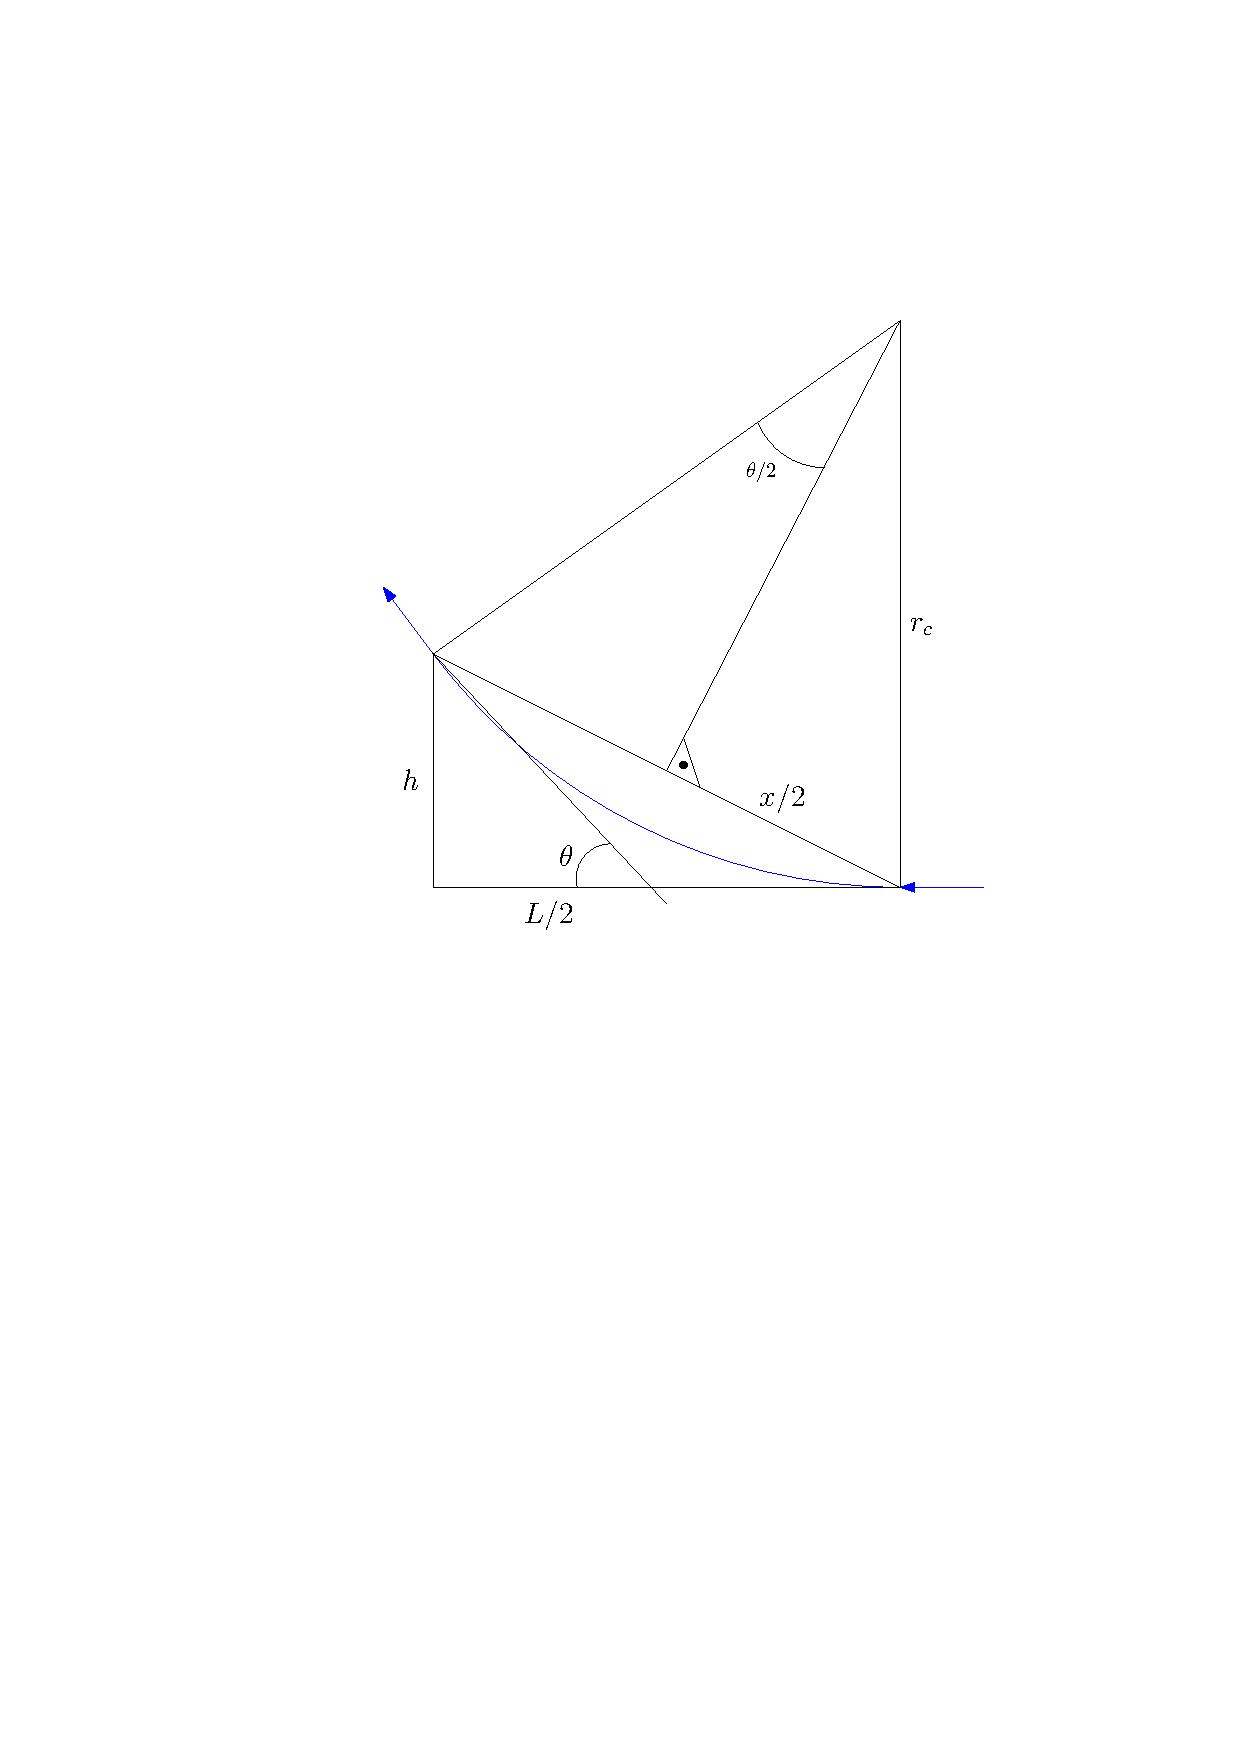
\includegraphics[width=0.5\textwidth]{\appdird/momentum.pdf}
    \caption{Two dimensional geometrical representation of a particle trajectory (blue) deflection in a uniform magnetic field.}
    \label{fig:momentumgeo}
\end{figure}
In the small angle approximation ($\sin\theta=\theta+\mathcal{O}(\theta^2)$ and $\tan\theta=\theta+\mathcal{O}(\theta^2)$), following quantities are defined:
\begin{equation}
  \label{eq:mom-simple}
        \sin\frac{\theta}{2}\simeq\frac{x}{2r_c},\hspace{5mm}
        \tan\theta\simeq\frac{2h}{L},\hspace{5mm}x=\sqrt{h^2+L^2}=h\sqrt{1+\left(\frac{L}{h}\right)^2}\Rightarrow r_c\simeq\frac{L}{2}\sqrt{1+\left(\frac{L}{h}\right)^2}
\end{equation}
Finally the radius is projected on the beam axis and the momentum is obtained from the well-known relation $p_\perp^\text{reco}=0.3eBr_c$. 
\subsection{Kalman filter}
\label{appD:sec:kalman-filter}

%%% Local Variables:
%%% mode: latex
%%% TeX-master: "../PhDthesis"
%%% End:
